\documentclass[a4paper]{article}

\usepackage[a4paper, margin=0.5in]{geometry}
\usepackage{graphicx}
\usepackage[linesnumbered,ruled,vlined]{algorithm2e}
\usepackage{color,soul}
\usepackage[utf8]{inputenc}
\usepackage[T1]{fontenc}
\usepackage{textcomp}
\usepackage{amsmath, amssymb}
\usepackage{caption}
\usepackage{listings}
\usepackage[italian]{babel}

% figure support
\usepackage{tikz}
\usetikzlibrary{calc}
\usepackage{import}
\usepackage{xifthen}
\pdfminorversion=7
\usepackage{pdfpages}
\usepackage{transparent}
\usepackage[hidelinks]{hyperref}
\usepackage{multirow}

% provides the H option
\usepackage{float}

\pdfsuppresswarningpagegroup=1

\begin{document}
	\title{Project log - Robotica}
	\author{Augello Andrea \and Castiglione Francesco Paolo \and La Martina Marco}
	\maketitle
	\tableofcontents

	\section{Setup}\label{sec:Setup}
	\begin{tabular}{|l|r|}
		\hline
		\multirow{2}{4em}{OS} & Ubuntu 18.04 \\
							  & Ubuntu 20.04 \\ \hline
		\multirow{2}{6em}{ROS version} & melodic \\
									   & noetic \\ \hline
		Webots & R2020b revision 1\\ \hline
		\multirow{2}{11em}{Target hardware} & Raspberry Pi 4B \\
											& Raspberry Pi 3B+ \\ \hline
	\end{tabular}

	\section{Nome}\label{sec:Nome}
	Il team ha scelto il nome \textbf{Change} in onore di \textbf{Chang'e 4} \cite{change4}, la missione parte della seconda fase del programma cinese di esplorazione lunare, durante il quale è andato a buon fine il primo atterraggio morbido sulla faccia nascosta della luna. 

	\section{Ambiente}\label{sec:Ambiente}
	Abbiamo considerato opportuno analizzare e studiare il package \textbf{webots\_ros} \cite{webotsRosSetup} al fine di raggiungere una comprensione più profonda sulle metodologie per interfacciare i nodi ROS con il controller ROS standard per Webots. Inoltre è risultato necessario approfondire la documentazione ROS \cite{ros.org} al fine di installare e configurare l'ambiente ROS ed inoltre per capire i concetti fondamentali relativi ai nodi e topics. Infine abbiamo impostato l'interfaccia ROS su Webots seguendo la documentazione cyberbotics rilevante \cite{ros.org}.
	
	\section{ROS}\label{sec:Ros}
	
	\subsection{Bug}\label{sec:Bug}
	Nel file RosSpeaker.cpp, parte del controllore ROS per Webots \cite{cyberbotics}, è stato riscontrato un bug. Il metodo per verificare che si sta riproducendo un suono da file audio ed il metodo per verificare che il robot sta parlando presentavano difatti le funzioni callback invertite. In seguito al nostro avviso via email il bug è stato risolto nel successivo aggiornamento, come si evince dal commit github rilevante \cite{rosbug}, riga 32-34.
	
	\section{Dipendenze}\label{sec:Dipendenze} 
	La seguente è una lista delle librerie utilizzate nel nostro progetto ed una breve spiegazione della loro funzione e rilevanza:
	
	\begin{itemize}
		\item opencv 4.x, una libreria per la computer vision, usata per operazioni di segmentazione \cite{opencv};
		\item imutils, che include funzioni per semplici operazioni di image processing quali traslazioni, rotazioni, ridimensionamento. Utilizzato inoltre per effettuare Non Maxima Suppression(NMS) \cite{imutils};
		\item sklearn, una libreria per il machine learning comprendente algoritmi di clustering quali DBSCAN \cite{scikit};
		\item numpy, una libreria che fornisce supporto per array multidimensionali, matrici ed operazioni matematiche per lavorare su detti array \cite{numpy};
		\item matplotlib, una libreria per creare visualizzazioni di dati (statiche, dinamiche, interattive) \cite{matplotlib};
		\item math, una libreria che fornisce funzioni matematiche definite dallo standard C \cite{math}.
	\end{itemize}

	\section{Obbiettivo}\label{sec:Obbiettivo} 
	L'obbiettivo del robot è di \textbf{evitare assembramenti in ambienti indoor}. \newline
	Nella dimostrazione presentata il nostro robot rileva le persone nella stanza e individua i possibili assembramenti. In seguito alla fase di rilevazione si sposterà verso l'assembramento evitando gli ostacoli e, arrivato, esorterà le persone al rispetto del distanziamento sociale.
	
	\section{TIAGo Iron}\label{sec:TIAGo-Iron} 
	Il robot scelto per l'obbiettivo proposto è il \textbf{TIAGo Iron}. \newline Il \textbf{PAL Robotics TIAGo Iron} \cite{tiagoiron} è un robot umanoide a due ruote con torso e testa ma senza braccia articolate. Il modello è una piattaforma modulare mobile che permette l'interazione fra esseri umani e robot. \newline
	Il datasheet del \textbf{TIAGo} indica la presenza di speaker e display, tuttavia questi non sono presenti nel modello Webots. Abbiamo dunque ritenuto necessario per il nostro scopo aggiungere uno \textbf{speaker} e un \textbf{display} con corrispondente solido di supporto al modello.
	La camera del \textbf{TIAGo}, come indicato dal datasheet, è RGB-D. Il modello Webots ne è sprovvisto, di conseguenza è stata utilizzata una camera monoscopica RGB.
	Inoltre è stato necessario contattare gli sviluppatori del \textbf{TIAGo} per chiedere informazioni circa le dimensioni esatte delle \textbf{ruote} in quanto tale informazione è omessa dal datasheet. Ci è stato comunicato che le ruote del \textbf{TIAGo} hanno raggio di $200\,mm$. Utilizzando tale valore nei calcoli odometrici, abbiamo ottenuto valori largamente differenti dalle misurazioni. Abbiamo quindi dedotto sperimentalmente che il raggio del modello Webots è di $3\,cm$ più lungo. 
	
    L'IMU utilizzata ha 6 gradi di libertà ed è composta delle seguenti componenti:
	\begin{enumerate}
		\item giroscopio;	
		\item accelerometro;
	\end{enumerate}
	Abbiamo ritenuto non necessario aggiungere il \textbf{magnetometro} in quanto in uno scenario reale sarebbe stato soggetto ad interferenze (significativamente più di un giroscopio), specialmente in un ambiente con molti oggetti metallici (quale potenzialmente lo scenario di utilizzo del nostro robot).
	
	Il modello Webots del \textbf{TIAGo} presenta uno slot libero per il lidar. Abbiamo scelto il modello Hokuyo URG-04LX-UG01 \cite{lidarspecs} che, come specificato dalla documentazione del modello Webots,  ha un range di $5.6\,m$ ed un FOV di $240^{\circ}$ (ricordiamo che agli estremi è parzialmente occluso).

	\section{Modello del moto e posizionamento}\label{sec:Modello-del-moto-e-posizionamento}
	Il modello del moto è caratterizzato da rotazioni e traslazioni. Per ottenere l'angolo di rotazione ci basiamo sui dati ottenuti dal giroscopio, il quale misura il moto rotazionale fornendo una velocità angolare. Per ottenere l'angolo di rotazione effettuiamo quindi un'integrazione discreta dei campioni con interpolazione lineare del primo ordine.
	Per effettuare lo spostamento lineare utilizziamo il controllore PID (Proporzionale-Integrale-Derivativo) delle ruote fornito da Webots, che richiede l'angolo di rotazione corrente, il diametro delle ruote e fornisce l'angolo di rotazione necessario al fine di ottenere lo spostamento desiderato.
	\begin{equation}\label{eq:odometry}
	targetAngle =
	currentAngle+2\pi\frac    {distance}
	{2\pi \cdot diameter}
	\end{equation}
	
	A causa di possibili imprecisioni calcoliamo la stima dello spostamento lineare utilizzando l'accelerometro. Al segnale dell'accelerometro viene applicato un integrale doppio per ottenere lo spostamento lineare.
	
	Nell'immagine seguente viene mostrata la zona nella quale, se viene indicata dal \textbf{lidar} la presenza di un ostacolo, il \textbf{TIAGo} si ferma per ragioni di sicurezza al fine di evitare danni a persone e/o oggetti.
	\begin{figure}[H]
		\centering
		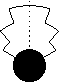
\includegraphics[width=0.2\textwidth]{./img/collision_detection.pdf}
		\caption{Collision detection}
		\label{fig:collision_detection}
	\end{figure}
	
	\section{Object recognition}\label{sec:Object-recognition}
	
	\subsection{Campionamento delle immagini}\label{subsec:Campionamento-delle-immagini}
	Il FOV della camera è di 57°, di conseguenza per ricoprire 360° è stato necessario effettuare 7 campionamenti. Il settimo campionamento, come si evince dalla figura \ref{fig:campionamento_immagini}, è sovrapposto al primo per una porzione di scena pari a 39° coincidente col primo campionamento.
	
	\begin{figure}[H]
		\centering
		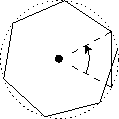
\includegraphics[width=0.4\textwidth]{./img/pictures_sampling.pdf}
		\caption{Campionamento delle immagini}
		\label{fig:campionamento_immagini}
	\end{figure}
	
	\subsection{Yolo}\label{subsec:Yolo}
	Al fine di riconoscere le persone è stato necessario utilizzare sistemi di \textbf{object recognition}. A tal fine abbiamo valutato le performance di YOLOv3 (you only look once), YOLOv3-tiny, HoG (Histogram of oriented gradients), HoG + SVG (support vector machines) + NMS (non maxima suppression).
	In seguito a vari test su HoG abbiamo ritenuto essere problematica la larghezza delle bounding boxes fornite, in quanto, per motivazioni che verranno chiarite nel paragrafo successivo, vogliamo che queste ultime siano il più possibili vicine alla reale larghezza delle persone. YOLOv3, nonostante sia stato addestrato su foto di persone reali (e non modelli 3D) fornisce risultati soddisfacenti, in seguito al finetuning degli iperparaemtri parametri della rete. Tuttavia, considerando le caratterisiche hardware del robot mobile, abbiamo optato per l'uso di YOLOv3-tiny, il quale risulta essere significativamente più efficiente, sacrificando in termini di precisione ma comunque sufficientemente preciso per il nostro obbiettivo. Ecco un paragone fra YOLOv3 e YOLOv3-tiny in termini di mAP (mean average precision) e FLOPS (floating-point operations per second), come illustrato dalla tabella seguente, i cui dati provengono dal sito di YOLO \cite{yolo}:
	
	\begin{center}
		\begin{tabular}{ |c|c|c|c| } 
			\hline
			Model & mAP & FLOPS & FPS \\
			\hline	
			 YOLOv3-320    & 51.5  &  38.97  Bn  &  45  \\ 
			 YOLOv3-416    & 55.3  &  65.86  Bn  &  35  \\ 
			 YOLOv3-608    & 57.9  &  140.69 Bn  &  20  \\ 
			 YOLOv3-tiny   & 33.1  &  5.56   Bn  &  220 \\
			 YOLOv3-spp    & 60.6  &  141.45 Bn  &  20  \\
			\hline
		\end{tabular}
	\end{center}

	\subsection{Scarto dei duplicati}\label{subsec:Scarto-dei-duplicati}
	Durante la fase di individuazione delle persone vengono individuate varie bounding box corrispondenti al medesimo individuo. Di conseguenza è stato necessario effettuare una fase di clustering al fine di scartare le bounding box duplicate. L'algoritmo di clustering utilizzato è DBSCAN (Density based scan) \cite{DBSCAN}, i cui parametri principali sono \textbf{eps}, ovvero la massima distanza fra due punti affinché vengano considerati appartenenti a un cluster (da non confondere con la massima distanza fra i punti di un cluster), \textbf{min\_samples}, ovvero il numero minimo di punti affinchè un cluster sia valido (nel nostro caso è uguale a 1 in quanto non vogliamo scartare ROI) ed infine la metrica di distanza. 
	Come di evince dalla figura \ref{fig:nms}, la metrica utilizzata considera la lunghezza di un arco di circonferenza con raggio corrispondente alla distanza fra i due punti ed angolo $\alpha$ corrispondente  all'angolo fra i due punti rispetto alla posizione del robot.
	
	Abbiamo ritenuto opportuno utilizzare l'implementazione dell'algoritmo fornita da \textbf{sklearn} \cite{scikit}.
	
	\begin{figure}[H]
		\centering
		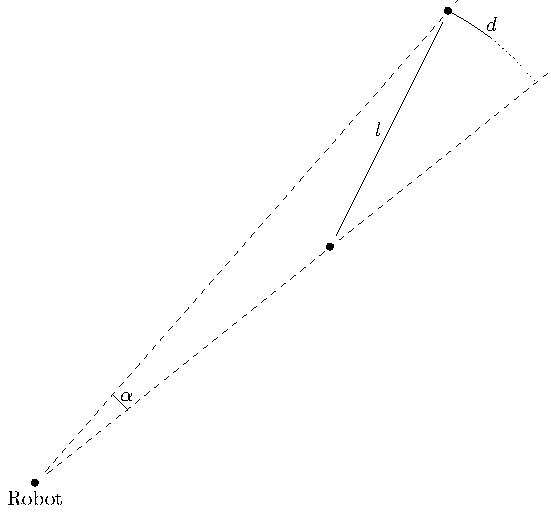
\includegraphics[width=0.6\textwidth]{./img/nms.pdf}
		\caption{Non maxima suppression}
		\label{fig:nms}
	\end{figure}
	\section{Posizione dei target}\label{sec:Posizione-dei-target}
	
	\subsection{Triangolazione}\label{subsec:Triangolazione}
	La triangolazione come metodo di individuazione delle persone, sebbene teoricamente possibile, presenta dei problemi nel nostro scenario. In primo luogo prendiamo in esame l'occlusione delle persone. Ad esempio, se due persone (5 e 2) sono una dietro l'altra lungo una retta immaginaria che le congiunge al robot (B), quest'ultimo non sarà in grado di individuare la persona 5. Inoltre, quando il robot effettua scan successivi, non sarebbe in grado di dedurre quali osservazioni derivano dalla stessa persona. Infatti, poiché nel nostro scenario abbiamo più persone in una stanza, non è possibile dedurre quali intersezioni delle rette corrispondono ad osservazioni reali o se si tratta di intersezioni spurie. 
	
	\begin{figure}[H]
		\centering
		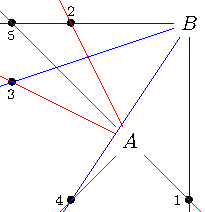
\includegraphics[width=0.5\textwidth]{./img/ideal_object_triangulation.pdf}
		\caption{Triangolazione}
		\label{fig:triangulation}
	\end{figure}
	
	\subsection{Calcolo della distanza}\label{subsec:Calcolo-della-distanza}
	
	L'altezza percepita dell'oggetto non è un indicatore affidabile della sua distanza dal robot in quanto parte dell'oggetto potrebbe essere occlusa o non presente nel frame. Inoltre classificatori quali HoG tendono a produrre ROI significativamente più alte dell'oggetto. La larghezza del torso, invece, è meno suscettibile a tali problemi, e non dipende dalla posizione (ad esempio seduto o alzato). Dobbiamo tuttavia ipotizzare che il torso abbia forma cilindrica introducendo quindi degli errori se l'obbiettivo non sta guardando la camera.	La posizione orizzontale dell'oggetto relativa alla camera può influenzare la larghezza percepita diminuendola quando aumenta la distanza dal centro dell'immagine. Ipotizzando che la camera abbia un FOV (field of view) di $2\alpha$ e sia distante $d$ dall'oggetto, la massima distanza orizzontale che un punto dell'immagine potrebbe avere dal centro del piano dell'immagine sarebbe $a = d \tan alpha$ (Fig.~\ref{fig:error}).
	
	\begin{figure}[H]
		\centering
		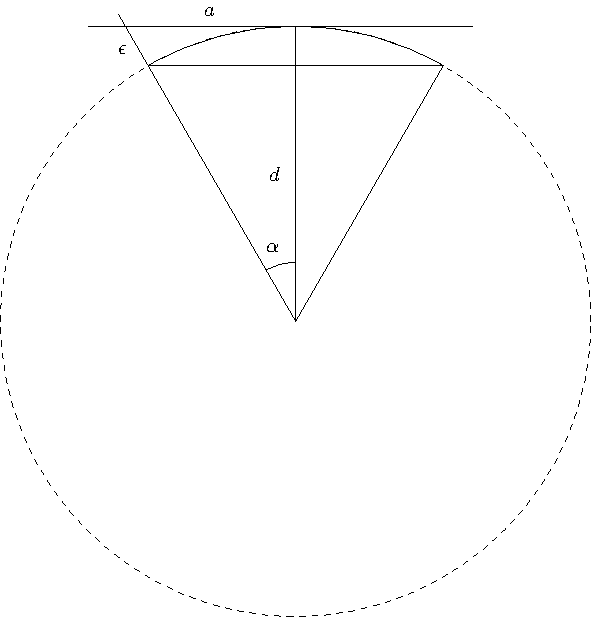
\includegraphics[width=0.8\textwidth]{./img/linearization_error.pdf}
		\caption{Errore nella stima della distanza con una linearizzazione a tratti della circonferenza}
		\label{fig:error}
	\end{figure}

	Ignorare la prospettiva significa effettuare un'approssimazione lineare del
	primo ordine e trattare il punto come se si trovasse su una circonferenza
	di raggio $d$ centrata sulla camera. Di conseguenza consideriamo il punto
	come se fosse più vicino di quanto non sia realmente, commettendo l'errore
	mostrato nell' Eq.~\ref{eq:max_err}. Con una camera con FOV di 1 radiante
	quale quella del TIAGo il massimo errore causato dalla linearizzazione è
	quindi una sottostima del 13.9\%.
	
	\begin{equation}
	\epsilon = 
	\sqrt{a^2+d^2} - d =
	\sqrt{(d\tan \theta )^2+d^2}-d =
	d\left( \sqrt{\frac{1}{\cos ^2 \alpha}}-1 \right) =
	d \left( \sec \alpha -1 \right) 
	\label{eq:max_err}
	\end{equation}
	
	Sotto tali ipotesi possiamo quindi calcolare la distanza di un oggetto come
	mostrato in Eq.~\ref{eq:obj_dist}
	
	\begin{equation}\label{eq:obj_dist}
	object~distance(m) = 
	\frac{f(m) \times real~width(m) \times image~width(pixels)}
	{object~width(pixels) \times sensor~width(m)}
	\end{equation}
	
	Poiché stiamo utilizzando un simulatore non è nota la larghezza del sensore
	da utilizzare per l'eq.~\ref{eq:obj_dist}. Abbiamo ovviato a tale problema
	posizionando il robot ed un oggetto dalle dimensioni note in posizioni note
	e abbiamo utilizzato questi dati insieme a delle misure in pixel nell'
	eq.~\ref{sensor_size}. Abbiamo così stimato le dimensioni del sensore
	virtuale da utilizzare nei calcoli successivi.

	\begin{equation}\label{sensor_size}
	sensor~width(m) = 
	\frac{f(m) \times real~width(m) \times image~width(pixels)}
	{object~width(pixels) \times object~distance(m)}
	\end{equation}
	
	\subsection{Modello probabilistico}\label{subsec:Modello-probabilistico}

	Le relazioni geometriche sulla distanza degli oggetti esposte nella
	sezione~\ref{subsec:Calcolo-della-distanza} assumono che il target abbia la
	stessa larghezza in ogni posa e che sia possibile ottenere dal
	classificatore delle bounding box estremamente aderenti all'oggetto. Dato che queste
	assunzioni non sono rispettate nella nostra applicazione la distanza
	dell'oggetto sarà soggetta ad errore non trascurabile. Per questa
	ragione e per i problemi legati alla triangolazione abbiamo abbandonato la
	rappresentazione basata su oggetti e abbiamo fatto ricorso ad un filtro di
	occupazione bayesiano (BOF)~\cite{tay2008bayesian}.

	Nelle classiche metodologie di tracciamento, il problema dell'associazione dei dati (data association), ovvero di associare un oggetto $o_t$ al tempo $t$ con un oggetto $o_t+1$ al tempo $t+1$, e della stima dello stato si configurano come classici problemi da risolvere. Nel filtro di occupazione bayesiano, il problema dell'associazione dei dati viene superato in quanto viene gestito da un livello di astrazione superiore. Il concetto di oggetto viene difatti riformulato da proprietà più utili quali occupazione o rischio, che vengono stimate direttamente per ogni cella utilizzando sia osservazioni dai sensori che conoscenze pregresse. Le caratteristiche di incertezza legate ai sensori vengono descritte, in questo modello, attraverso le probabilità di occupazione.

	Al fine di trasformare le osservazioni ottenute in una probabilità che le
	persone si trovino effettivamente nella posizione indicata è stato
	necessario definire una funzione densità di probabilità. La distribuzione
	normale, sebbene relativamente appropriata nel nostro scenario, è
	computazionalmente onerosa. La griglia di occupazione ha diverse migliaia
	di celle per cui va calcolata una pdf per ogni osservazione. Come si evince
	dalla fig.~\ref{fig:pdf_benchmark} con un numero così elevato di iterazioni
	i tempi di esecuzione non sarebbero accettabili, è stato quindi necessario
	ricorrere ad una approssimazione.
	
	\begin{figure}[H]
		\centering
		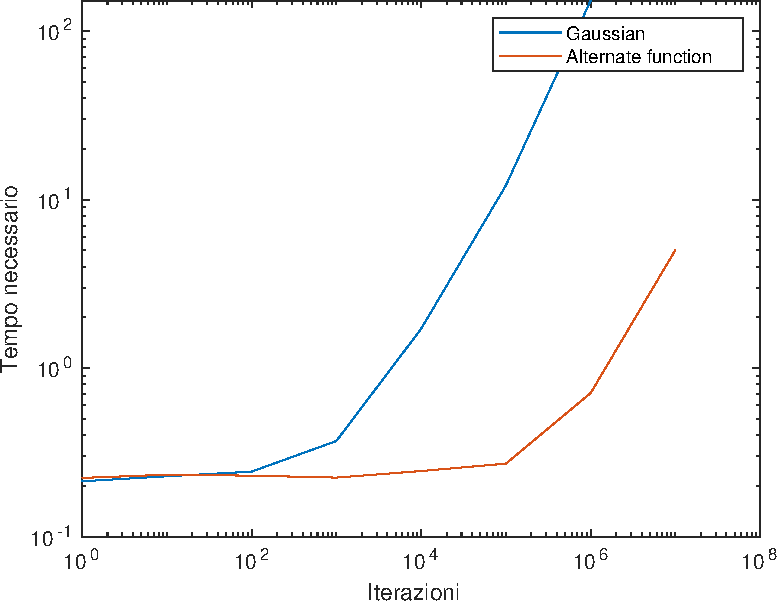
\includegraphics[width=0.6\textwidth]{./img/pdf_benchmark.pdf}
		\caption{Benchmark funzione densità di probabilità (probability density function, funzione )}
		\label{fig:pdf_benchmark}
	\end{figure}

	Un'approssimazione di largo uso è la distribuzione triangolare.
	Quest'ultima, tuttavia, presenta delle caratteristiche non desiderabili per
	il nostro caso d'uso. Una proprietà desiderabile della nostra funzione,
	difatti, sono le "fat tails", ovvero le code della distribuzione devono
	essere spesse e la distribuzione non deve tagliare nettamente. Quando, in
	seguito ad un'osservazione, non abbiamo alcuna osservazione di conferma
	nello scan successivo, non è infatti desiderabile che la probabilità di
	trovare una persona in quel punto scenda a zero. Inoltre, in una prima
	osservazione, un oggetto potrebbe essere occluso ed essere rilevato solo
	successivamente, quindi se in quella zona la probabilità di rilevare un
	target scendesse a zero non sarebbe possibile integrare correttamente
	questa nuova informazione. Ulteriori complicazioni sorgerebbero in caso di
	target in movimento.
	
	Essendo la scansione una operazione estremamente costosa non è nemmeno
	possibile affidarsi esclusivamente all'aggiunta di rumore alla griglia di
	occupazione confidando in una eventuale convergenza.

	Al fine di ottene un'approssimazione di una gaussiana adatta al
	nostro scenario, per modellare la probabilità che data l'occupazione della
	cella in posizione $ {\bf x} $ si ottenga l'osservazione $ {\bf z} $ è
	stato utilizzato un funzionale ispirato al guadagno del filtro di
	Butterworth.
	\begin{equation}\label{eq:pdf}
		p({\bf z}|{\bf x}) = \frac	{K}
		{1 + d({\bf x},{\bf z})^4 } 
	\end{equation}
	Nell'equazione~\ref{eq:pdf} è mostrato il funzionale utilizzato. In
	figura~\ref{fig:pdf_shape} si mostra un confronto della forma di questa
	funzione rispetto ad una gaussiana con media nulla e deviazione standard
	unitaria nel caso monodimensionale.
	
	Nell'equazione~\ref{eq:pdf} $K$ indica un parametro di scala per ottenere
	CDF unitaria. $d$ è una funzione per il calcolo della distanza della cella
	$ {\bf x} $ dalla stima di posizione $ {\bf z} $.

	La distanza euclidea porterebbe a formare aree ad alta probabilità di forma
	circolare. Questo però non si adatta bene al nostro modello di errore del
	sensore: l'angolo dell'oggetto rispetto al robot è noto con una precisione
	molto elevata, mentre la maggior parte dell'incertezza si concentra nella
	distanza. Utilizziamo quindi la distanza di Mahalanobis per tenere conto
	del nostro modello.

	\begin{figure}[H]
		\centering
		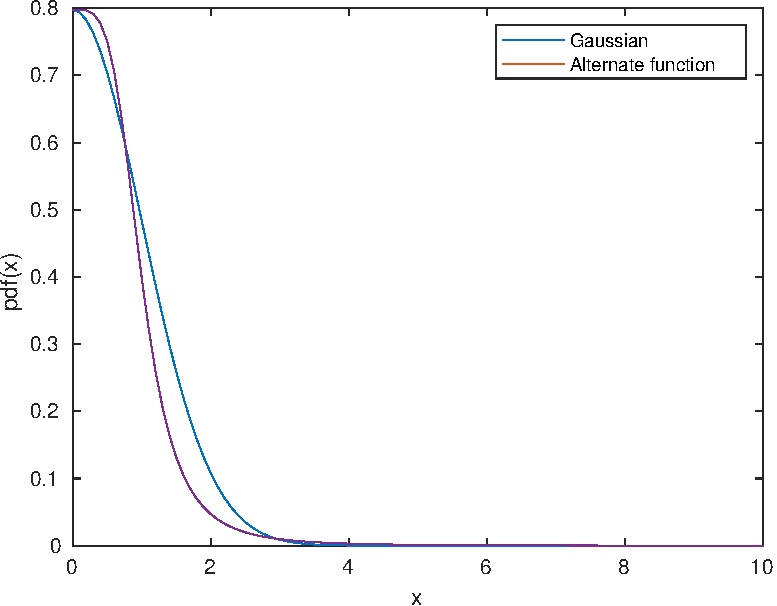
\includegraphics[width=0.6\textwidth]{./img/pdf_shape.pdf}
		\caption{Forma pdf}
		\label{fig:pdf_shape}
	\end{figure}

	Dato un insieme di osservazioni ottenute da una scansione $ Z_i $ aggiorniamo il belief precedente rispetto ad ogni cella della griglia di occupazione come mostrato nell'equazione~\ref{eq:belief-update}.

	\hl{TODO: check math to match slides}

	\begin{equation}\label{eq:belief-update}
		p({\bf x}_i | Z_i) = p({\bf x}_{i-1}) \cdot 
		\sum_{{\bf z} \in Z_i} p({\bf z} | {\bf x})
	\end{equation}
	Al termine di ogni aggiornamento della mappa l'intera griglia viene inoltre
	normalizzata per avere somma unitaria.  
	Questa formula è valida sotto le seguenti assunzioni:
	\begin{itemize}
		\item In uno stesso scan osservazioni separate si riferiscono ad
			oggetti distinti. In altre parole date due osservazioni $z_1$ e
			$z_2$ queste non hanno intersezione, quindi $ p(z_1 \cup pz_2) =
			p(z_1)+p(z_2)-p( z_1 \cap z_2) = p(z_1)+p(z_2) $ 

			Questa assunzione è ragionevole ricordando che lo scan avviene
			ruotando intorno al centro del robot e che viene effettuato uno
			scarto dei duplicati tenendo conto dell'angolo, quindi non possono
			esserci due osservazioni distinte derivanti dall'occupazione della
			stessa posizione nella mappa.

		\item In assenza di nuove osservazioni la stima dello stato del sistema
			rimane invariata: $ \overline{bel}(x_i) = bel(x_{i-1}) $ 

			Il robot non si muove abbastanza velocemente da poter inseguire e
			raggiungere assembramenti di breve durata, ha senso quindi
			limitarsi a considerare situazioni prevalentemente stazionarie e
			assumere consistenza dell'ambiente tra uno scan e l'altro. Inoltre
			gli scan sarebbero comunque troppo infrequenti per ottenere stime
			significative sul movimento degli oggetti.

	\end{itemize}

	In pratica applicando direttamente queste formule si introdurrebbe un
	errore nell'interpretazione delle informazioni: se per qualche ragione in
	uno scan non venisse rilevato nessun oggetto, $ Z_i $ sarebbe l'insieme
	vuoto. In mancanza di nuovi dati si potrebbero tentare due approcci:
	resettare le stime o lasciarle del tutto invariate. Nessuno di questi
	approcci si dimostra soddisfacente:
	\begin{itemize} 
		\item Lasciare invariato il belief a seguito di multiple scansioni
			senza successo porterebbe a non notare che tutte le persone
			nell'ambiente in cui ci si trova sono andate via, continuando a
			considerare valide tutte le posizioni precedenti.
		\item Dall'altro lato, un approccio troppo drastico quale
			immediatamente scartare tutte le precedenti stime porterebbe a
			perdere informazioni utili a causa di occlusioni temporanee (e.g.
			il robot entra in una stanza vuota).
	\end{itemize}

	Per gestire questa situazione effettuiamo uno smoothing degli istogrammi
	prima di ogni update essendoci una diminuzione della certezza delle misure.
	Aggiungiamo inoltre del rumore. In questo modo in assenza di osservazioni
	ci sarà una tendenza al ritorno ad uno stato iniziale, ma sarà graduale in
	modo da evitare di scartare troppo rapidamente le informazioni pregresse.

	Al fine di individuare le zone con alta probabilità di contenere persone
	abbiamo utilizzato un approccio derivante dall'elaborazione delle immagini.
	In primo luogo separiamo i punti nella mappa in punti ad alta probabilità
	di essere occupati da persone e punti con bassa probabilità. Per effettuare
	questa sogliatura abbiamo utilizzato il metodo Otsu~\cite{otsu}, il quale
	applica un thresholding automatico calcolato minimizzando la varianza dei
	valori di intensità all'interno delle classi e massimizzandola fra classi
	differenti all'immagine in input.  
	
	Da questa sogliatura otteniamo una mappa binaria in cui sono evidenziate le
	celle ad alta probabilità. Applicando l'algoritmo in~\cite{contours},
	implementato in OpenCV, estraiamo le regioni ad alta probabilità contigue
	ed i loro contorni. Per ogni regione verrà selezionato come centro il punto
	con maggiore probabilità (Fig.~\ref{fig:image_segmentation}).

	\begin{figure}[H]
		\centering
		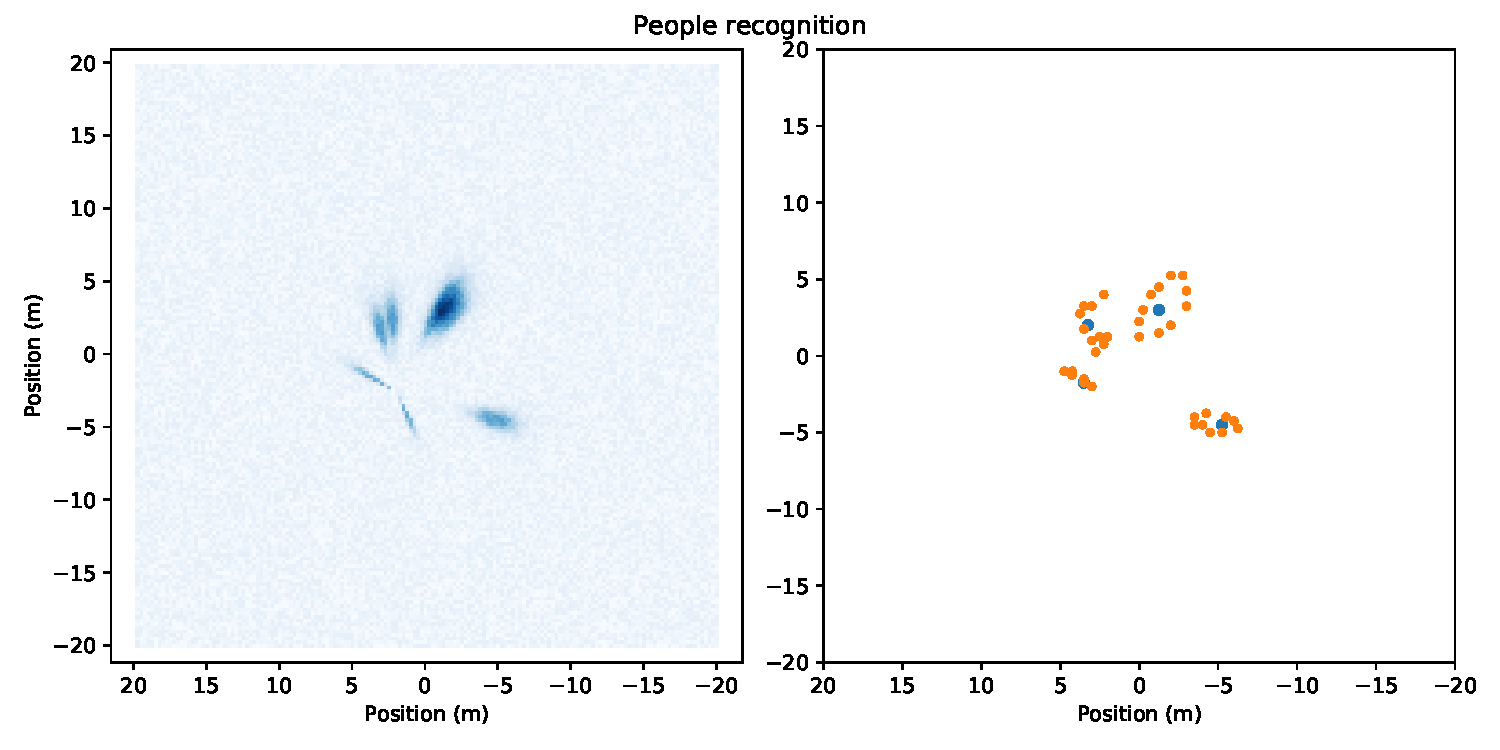
\includegraphics[width=1\textwidth]{./img/image_segmentation.pdf}
		\caption{Segmentazione immagine: a sinistra i valori grezzi del BOF, a destra i contorni delle regioni (giallo) e i centri (blu) }
		\label{fig:image_segmentation}
	\end{figure}
		
	\section{Pianificazione del moto}\label{sec:Pianificazione-del-moto}
	
	\subsection{Modalità di movimento}\label{subsec:Modalità-di-movimento}
	
	\subsubsection{Modalità esplorazione}
	Quando il robot entra in modalità esplorazione il suo comportamento è di esplorazione casuale della mappa. Il robot continua ad esplorare ed effettuare scan periodici fino a quando non viene rilevato un obbiettivo. In tal caso il robot entra in modalità campi di potenziale. Se il robot incontra un ostacolo nel suo cammino ruota di $90^{\circ}$ nella direzione opposta a quest'ultimo e continua l'esplorazione casuale.
	
	\subsubsection{Bug mode}
	Quando il robot entra in modalità bug effettuiamo uno scan lidar. Poiché lavoriamo con valori discreti, confrontiamo i valori ottenuti con una soglia al fine di individuare le discontinuità nel profilo degli oggetti nel range. Analizziamo successivamente le discontinuità del segnale, corrispondenti ai bordi degli ostacoli, come si evince dalla fig. \ref{fig:bug}. Da tali punti viene calcolato l'angolo fra la retta che li congiunge con l'obbiettivo. Il robot si muove infine verso il punto al quale corrisponde l'angolo minore, che ci farà allontanare meno dall'obbiettivo. Se il profilo dell'ostacolo è una circonferenza, la retta fra il punto con angolo minimo e l'obbiettivo è tangente all'ostacolo, da cui il nome dell'algoritmo Tangent Bug \cite{503814}.
	
	\begin{figure}[H]
		\centering
		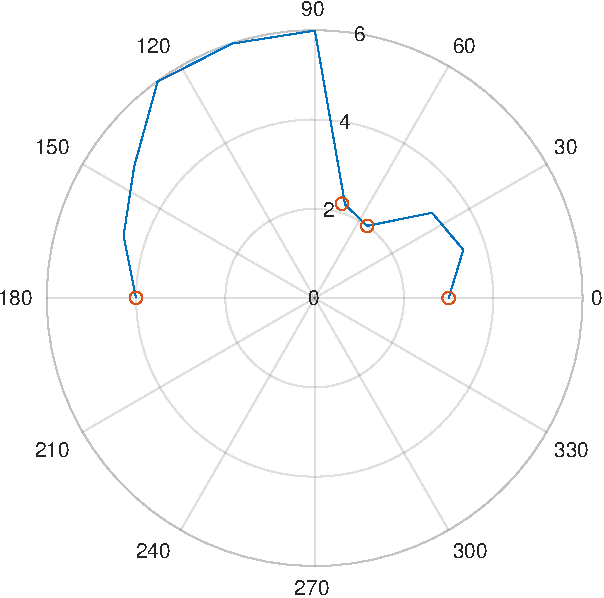
\includegraphics[width=0.4\textwidth]{./img/bug.pdf}
		\caption{Profilo dell'ostacolo}
		\label{fig:bug}
	\end{figure}

	\subsubsection{Campi di potenziale}
	
	
	\subsection{Pianificazione}\label{subsec:Pianificazione}
	\begin{figure}[H]
		\centering
		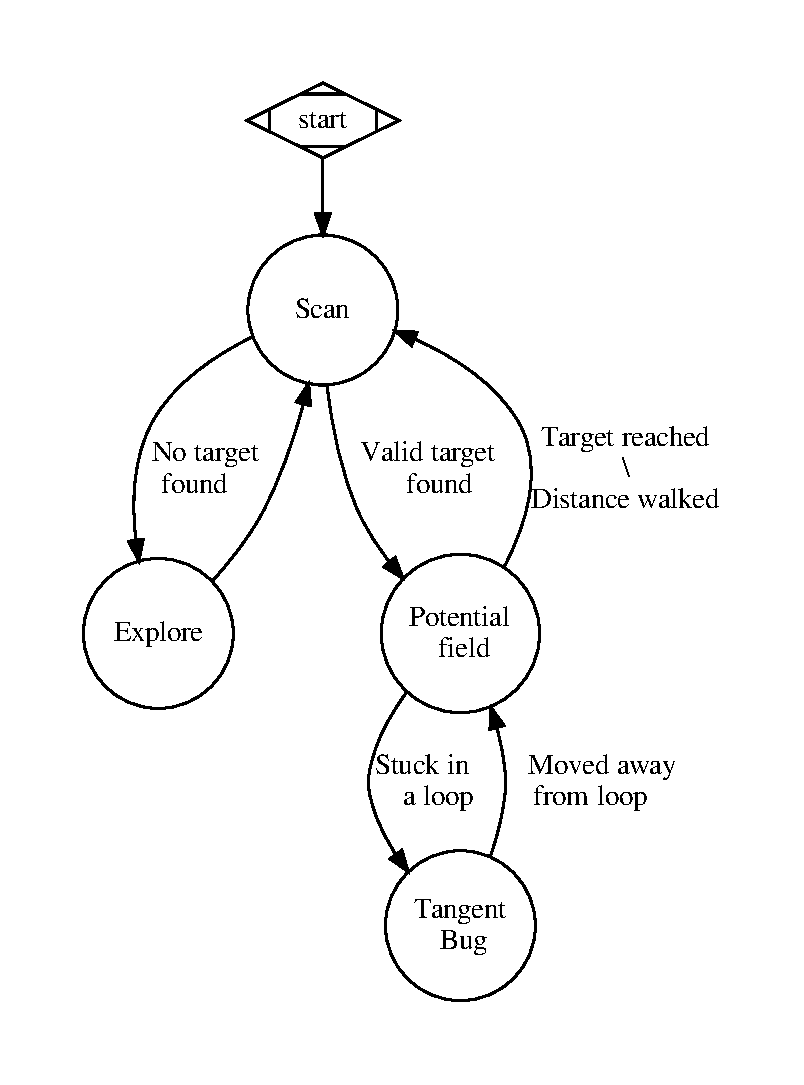
\includegraphics[width=0.6\textwidth]{./img/fsa.pdf}
		\caption{Automa a stati finito (Finite state automata)}
		\label{fig:fsa}
	\end{figure}
	
	\newpage
    % Bibliography
	\bibliographystyle{unsrt}
	\bibliography{references.bib}.

\end{document}
